\section{Evaluation}
\FloatBarrier%

For evaluation, two models are considered:
\begin{itemize}
  \item ``Baseline'', a basic convolutional neural network without using the
    clustering information.
  \item ``K-Means'', similar to the baseline model with the addition of
    clustering information into the final classification step.
\end{itemize}
These models are tested based on two scenarios that differ in the source of the
test set. In the first scenario, training and testing data are both pulled from
the same pool of data. In the second scenario, all the training data is
pulled from the most recent 18th electoral period, while the testing data comes
from a number of files from electoral periods 13, 14, 16 and 17. This makes the
problem more difficult in two ways:
\begin{enumerate}
  \item A change of electoral period means at least a partial change in
    parliamentary members, which reduces the ability of the model to essentially
    overfit on the names of members.
  \item Although older documents use the same layout as newer ones, the PDF
    files were generated using different software (electoral period 13 started
    in 1994 and was the first period to use truly  digital documents --- older
    documents are scanned versions of printed paper). This results in the flaky
    PDF decompiler making different mistakes than it does on the newer
    documents. This is a huge problem for rule-based systems; hopefully the
    probabilistic nature of machine learning makes it more robust to this issue.
\end{enumerate}
In the first scenario, the experiments are run 10 times using a \emph{shuffle
split} algorithm; this is similar to k-fold cross validation, but without the
restriction of having to use $k$ evenly sized splits. Instead, for each
iteration $n$ training samples are randomly sampled while the rest of the
samples are used for testing. The second scenario uses the same method for
generated a training set, but uses a separate, unchanging test set instead.
Additionally, the sampling is stratified, meaning it maintains the ratio (1:1)
of positive to negative samples in the dataset.

Before directly comparing the two models, a good baseline value has to be
determined for the two parameters in the model that are the most difficult to
determine:
\begin{enumerate}
  \item the size of the sliding window applied to the input data
  \item the number of clusters to detect in the blocks of text (i.e.\ the ``k''
    in k-means)
\end{enumerate}
Although there are more parameters, they are related to the convolutional
neural network; this means they can be set to pretty good values using prior
knowledge, as well as the fact that convolutional neural networks are not hugely
sensitive to their parameters.

\subsection{Sliding Window Size}
The effect of the sliding window size is explored
in \cref{fig:window_new,fig:window_old}. Both cases show a clear downward trend as
the window gets bigger, but peak at a different value. When testing on the full
dataset a very small window size of 2 performs best, while testing on older
electoral periods seems to require a bit more information and performs optimally
at a size of 4. In addition, both testing scenarios show the same behaviour
regarding the baseline and K-Means models: the K-Means model generally
outperforms the baseline at suboptimal window sizes, but at the optimum their
performance appears to be identical.
\begin{figure}[p]
  \centering
  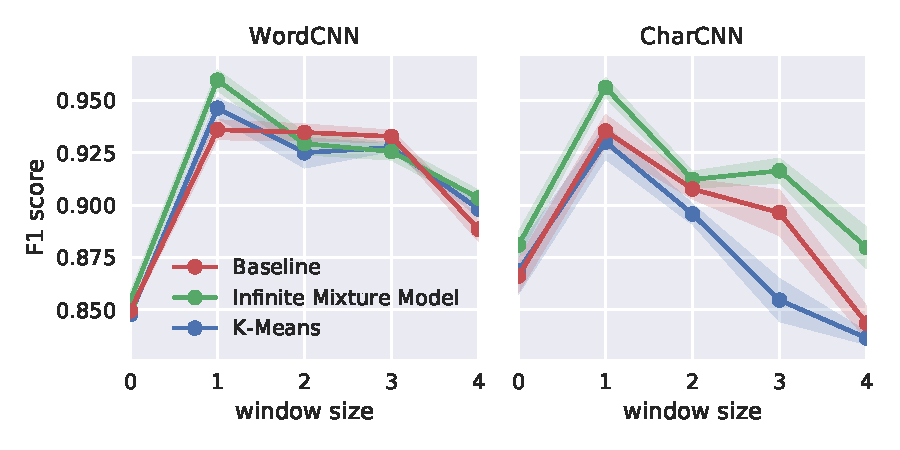
\includegraphics[width=\textwidth]{figures/results/2000-windowsize-old/tseries_f1.pdf}
  \caption{These figures shows the F1 score with regards to the sliding window
    size for each model trained on 2000 training samples.  The vertical axis
    shows the F1 score, averaged over 5 trials; the horizontal axis shows the
    size of the sliding window applied to the training data. The translucent
    bands around the lines indicates the confidence intervals, meaning that
    based on the observed F1 scores and assuming normality, the true mean is
    95\% likely to fall within that interval. The dots on the lines indicate
    measurements.\label{fig:window}}
\end{figure}

\subsection{Number of Clusters}
Results for the number of clusters are given in \cref{fig:numcluster}. In
this case, the window size was fixed to the previously determined optimum of 5.
The \texttt{Baseline} model was not tested due to it not using the clustering
data.  Although the results seem all over the place with large confidence
intervals, this is a bit of an illusion caused by the small range of F1 scores
that they span. There is an odd spike at 7 clusters which is hard to explain,
but might be caused by the probabilistic nature of the K-Means algorithm and the
fact that the same clustering was used for each trial; the particular K-Means
run when doing 7 clusters might have produced a below-average result.
\begin{figure}[tb]
  \centering
  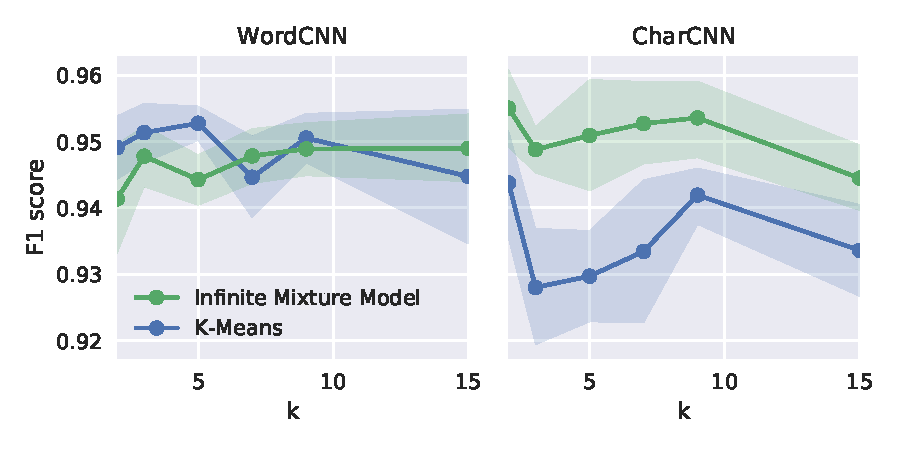
\includegraphics[width=\textwidth]{figures/results/2000-numclusters-old/tseries_f1.pdf}
  \caption{This figure shows the performance with regards to the number of
    cluster types for each model trained on 1200 training samples with a window
    size of 5.  The vertical axis shows the F1 score, averaged over 10 trials;
    the horizontal axis shows the number of cluster types considered in the
    final clustering step.  The translucent bands around the lines indicates the
    confidence intervals, meaning that based on the observed F1 scores and
    assuming normality, the true mean is 95\% likely to fall within that interval.
    The dots on the lines indicate measurements.\label{fig:numcluster}}
\end{figure}

\subsection{Training Set Size}
The results of all three models tested with the basic parameters
(\cref{tbl:params}) on various input sizes is shown in \cref{fig:result}. The
K-Means model outperforms the baseline at every input size, and as expected more
data greatly improves the performance, rising sharply up to 800 samples and
rising more gradually from then on. The precise values are given in
\cref{tbl:main}, along with $p$-values calculated through a two-tailed Student's
T-test.
\begin{figure}[tb]
  \centering
  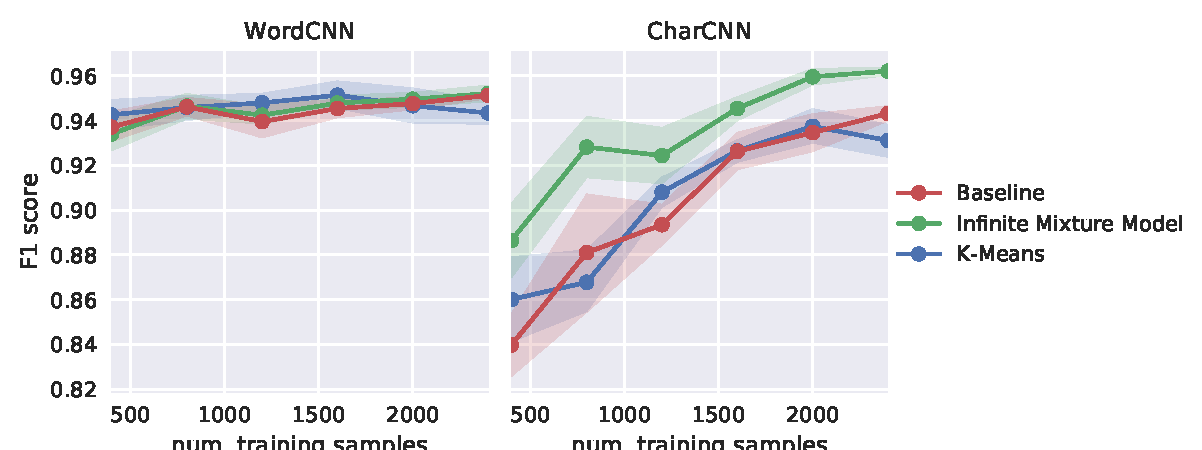
\includegraphics[width=\textwidth]{figures/results/training-size-old/tseries_f1.pdf}
  \caption{This figure compares the performance of the baseline model, using
    only a CNN, to that of the model augmented with K-Means clustering.  Tested
    on a test set of older electoral periods not present in the training set.
    The vertical axis shows the F1 score, averaged over 10 trials. The
    horizontal axis shows the number of samples used for training (at a 1:1
    ratio of positive to negative samples). The vertical bars indicate
    confidence intervals, meaning that based on the observed F1 scores and
    assuming normality, the true mean is 95\% likely to fall within the shown
  interval.\label{fig:result_old}}
\end{figure}

\begin{table}[tb]
  \centering
  \sisetup{%
    table-number-alignment = right,
    table-figures-integer  = 1,
    table-figures-decimal  = 4,
    table-unit-alignment   = center,
    detect-all             = true
  }
  \robustify\bfseries
  \robustify\em
  \begin{tabular}{l
    S[table-auto-round]
    S[table-auto-round]
    S[table-auto-round]
    S[table-auto-round]
    S[table-auto-round]
  }
    \toprule
    %\multirow{3}[5]{*}{Num.\ training samples} & \multicolumn{4}{c}{F1 Score} & \multirow{3}[5]{*}{p-value} \\
    \cmidrule(lr){2-5}
    & \multicolumn{2}{c}{Baseline} & \multicolumn{2}{c}{K-Means} & \\
    \cmidrule(lr){2-3} \cmidrule(lr){4-5}
    & {mean} & {std} & {mean} & {std} & \\
    \midrule
    50   & 0.826324 & 0.0239358  & \bfseries 0.834709 & 0.0266555  & 0.198132 \\
    100  & 0.860648 & 0.0222256  & \bfseries 0.86601  & 0.023512   & 0.344911 \\
    400  & 0.926813 & 0.00858367 & \bfseries 0.936305 & 0.00750224 & \em\/0.00477517 \\
    800  & 0.949605 & 0.00315041 & \bfseries 0.951964 & 0.00422667 & 0.0512679 \\
    1200 & 0.951701 & 0.00383244 & \bfseries 0.954277 & 0.0034699  & \em 0.0470661 \\
    1600 & 0.957737 & 0.00458451 & \bfseries 0.959859 & 0.00520081 & \em\/0.0496447 \\
    \bottomrule
  \end{tabular}
  \caption{The F1 scores of both models compared at different sizes of the
    training set. The reported means and standard deviations are based on 10
    repeated trials on randomized subsets of the data, with the higher mean
    between the two models bolded for emphasis. The last column indicates the
    probability that the scores for the K-Means model are drawn from the same
    distribution as those for the Baseline model (i.e.\ that their performance
    is the same and any observed difference is due to chance); probabilities
    below the usual $0.0.5$ cutoff for significance are rendered italic.\label{tbl:main}}
\end{table}

\FloatBarrier%

%%% Local Variables:
%%% mode: latex
%%% TeX-master: "report"
%%% End:
